\chapter{系统的架构建模及协同仿真可信性检测}
\label{ch3}
在本章节,我们首先用SysML建模语言对整个异构系统的架构进行建模,其中用SysML的BDD图来建模系统的组件,用SysML的IBD图来建模系统中各个组件之间的关联关系。由于SysML只是用来建模系统的架构,该建模语言得到的模型不可执行。因此,我们基于FMI标准,根据SysML的BDD描述的组件生成FMU模型(可以参考SysML建模的BDD图,使用FMUSDK等工具手动实现FMU;或是先用其他建模工具建模SysML描述的系统模型,然后导出FMU,例如Modelica、simulink等工具),根据SysML的IBD图生成FMU之间的接口配置文件。因此,我们只需要设计协同仿真主算法就可以完成系统中各个组件基于FMI的协同仿真。然而,在我们将基于FMI的协同仿真模型输入到协同仿真引擎之中进行仿真之前,我们需要确保该协同仿真模型的可信性,即要保证该模型可以正确的进行协同仿真并能得到正确的仿真结果。为了解决这个问题,我们需要对该协同仿真模型进行两个方面的可信性检测:(1)我们要检测协同仿真过程中使用的主算法的可信性,即主算法没有出现死锁以及其他一些不可信的特性;(2)我们要检测系统中各个FMU之间依赖关系及数据交互的可信性,其中最主要的要保证多个FMU之间没有出现环路依赖\cite{Broman2013Determinate}。由于协同仿真的过程及FMU的执行都是基于时间的,而时间自动机在建模时间行为上具有较大的优势,且对于时间自动机的可信性检测有着良好的工具支持。因此,在接下来的内容中,我们将重点描述如何基于时间自动机理论来检测模型协同仿真过程的可信性。在第一小节,我们给出模型协同仿真的可信性检测中使用的技术框架;第二小节介绍如何对上述的第一个方面,即协同仿真主算法进行可信性检测;在第三小节中,我们使用一个具体的案例来描述如何对上述的第二个方面进行验证,即协同仿真模型数据交换及依赖关系的可信性检测。
\section{技术框架}
\begin{figure}[htbp]
	\centering
	{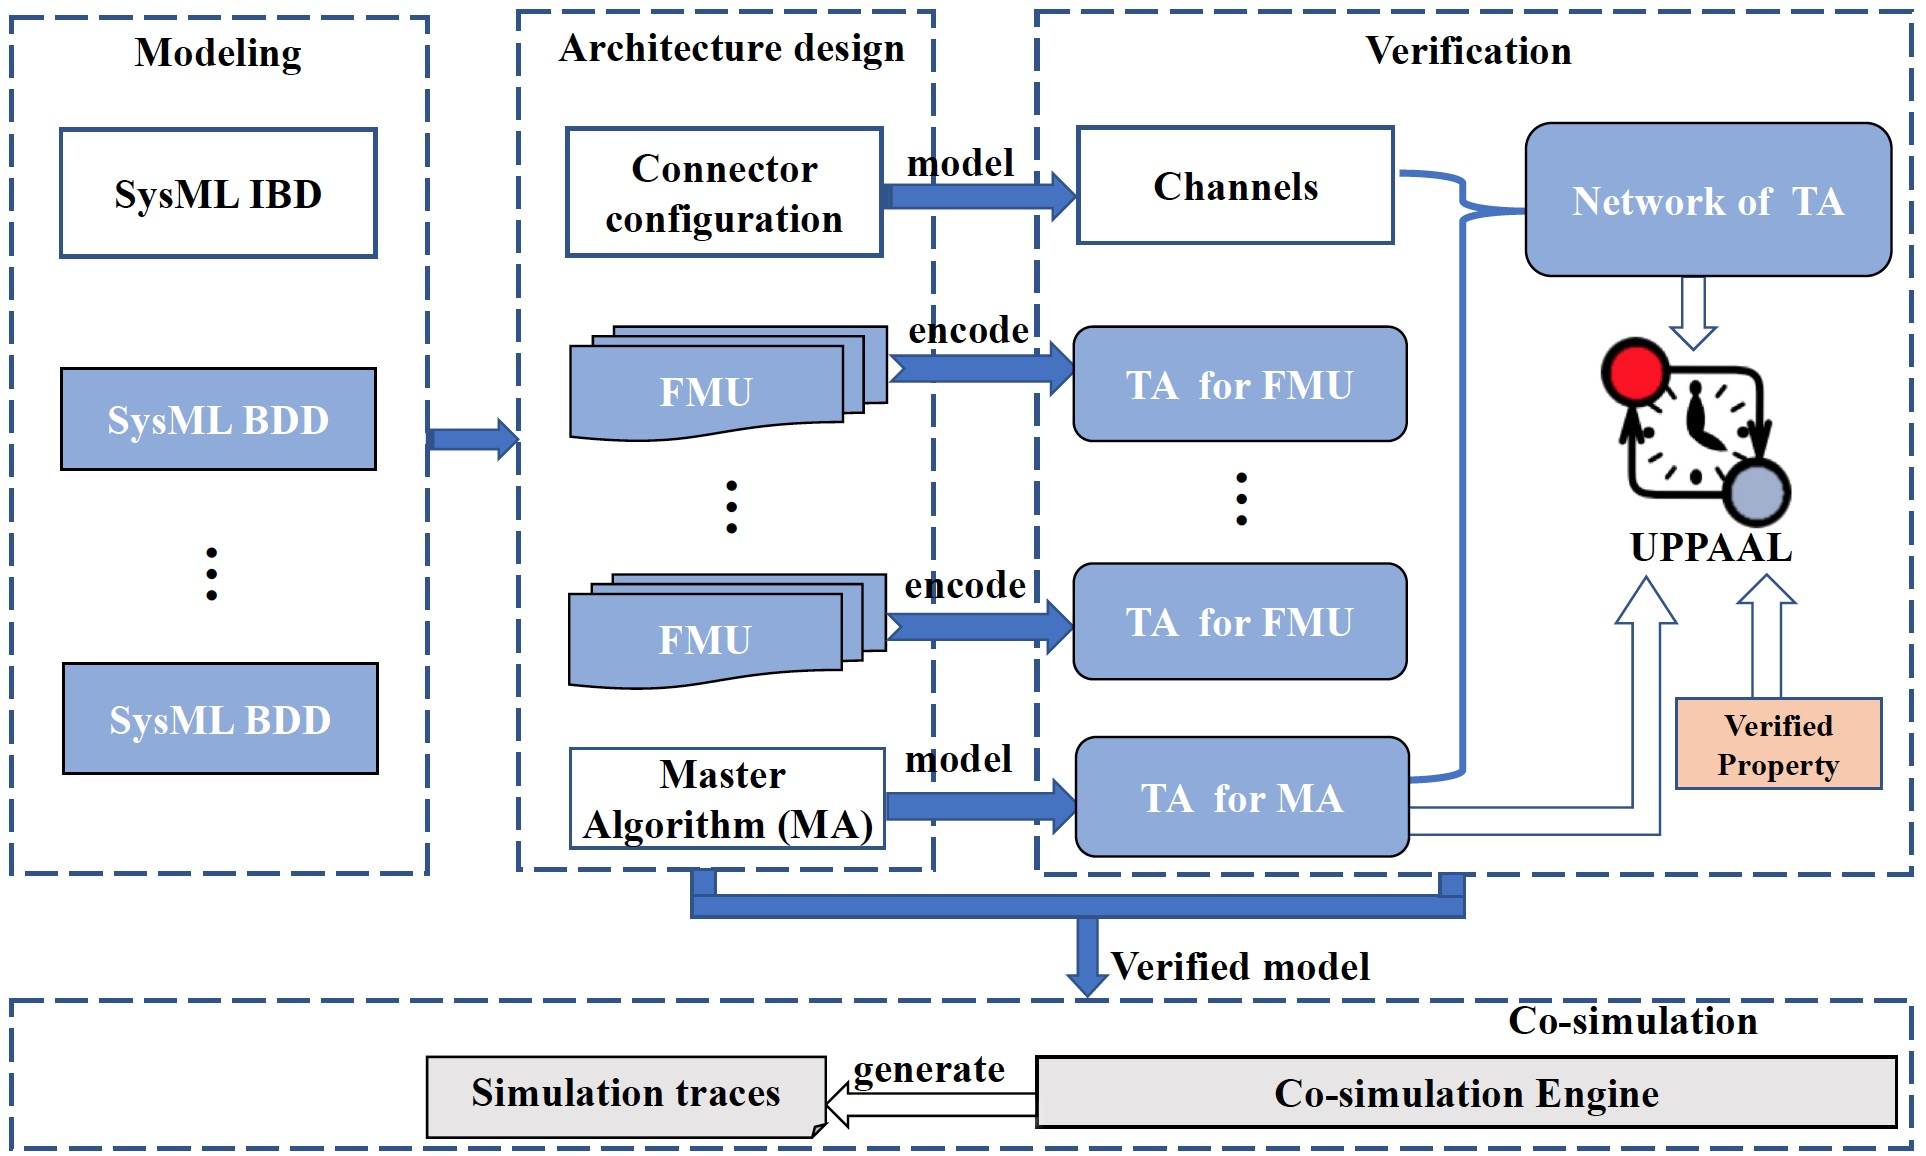
\includegraphics[width=6.0in]{fig/3/framework-3.png}}
	%\vspace{0.10in}
	\caption{协同仿真可信性检测的技术框架图}\label{fra-3}
\end{figure}
图\ref{fra-3}为系统协同仿真可信性检测的技术框架图。首先,我们在建模(Modeling)阶段使用SysML的BDD和IBD图来建模整个系统的架构,SysML BDD中的块建模了系统的各个组件;SysML的IBD(描述了各个块之间的连接关系。为了借助基于FMI的协同仿真技术对整个系统进行协同仿真,我们在架构设计(Architecture design)阶段根据BDD中描述的各个块生成对应的FMU,同时根据IBD图描述的关联关系生成FMU之间的连接配置文件(Connector configuration)。接下来,我们设计了协同仿真的主算法(Master Algorithm,MA)来实现各个FMU之间的交互,同时来驱动协同仿真过程的执行。接下来是协同仿真可信性检测(Verification)阶段,也是我们本文的主要贡献点之一。为了检测模型协同仿真行为的可信性,(1)我们先检测了协同仿真主算法的可信性:首先我们用时间自动机(TA)对协同仿真的主算法进行形式化建模,然后将建模得到的时间自动机模型输入到UPPAAL模型检测工具中,针对特定的属性(Verified Property)进行检测 ;(2)我们检测了协同仿真模型数据交换及依赖关系的可信性:首先我们提出了一种从FMU到时间自动机的映射规则,我们根据此映射规则将FMU映射为时间自动机,接下来将FMU之间的连接配置文件转化为时间自动机之间的通道(Channels)。这样,我们就得到了一个时间自动机网络(Network of TA):包括FMU映射成的时间自动机模型、主算法的时间自动机模型及各个时间自动机模型之间的通道)。最后我们将该时间自动机网络和要检测的属性(死锁、可达性、活性等)输入到UPPAAL中来检测该模型是否满足这些属性。一旦通过了协同仿真的检测可信性,我们就可以将通过检测的模型(Verified model)输入到协同仿真的引擎之中进行协同仿真并得到协同仿真的迹;如果未能通过协同仿真的可信性检测,我们则需要对模型进行修改,直到修改之后的模型通过可信性检测之后再对模型进行仿真。接下来,我们将详细介绍整个协同仿真可信性检测的过程。
\section{协同仿真主算法的可信性检测}
在本小节我们首先介绍了三种协同仿真的主算法:固定步长算法\cite{Bastian2011Master}、可回滚算法及可预测步长算法\cite{Broman2013Determinate},之后我们用时间自动机形式化建模了这几种算法,最后将这几种算法的形式化模型输入到UPPAAL工具中,分别检测了这几种算法的有无死锁及可达性和活性。
\subsection{协同仿真主算法介绍}
协同仿真的主算法用于调度和协同系统的多个FMU组件的执行。每一个FMU都可以被看做为一个可独立仿真的黑盒,但是多个FMU之间在某些特定的时刻需要进行数据交互和同步。图\ref{ad-fixedstep}为当前三种主要的协同仿真主算法的活动图。在接下来的内容中,我们将对这三种算法进行简单的介绍。
\begin{figure}[htbp]
\centering{
		\subfigure[固定步长算法]{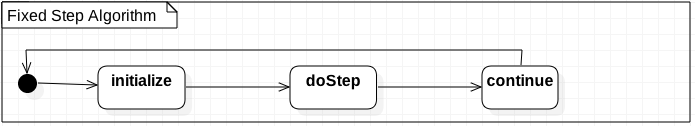
\includegraphics[width=4.5in,height=0.8in]{fig/3/MA1.png}
			\label{sd_fixedstep}}
		\hfil
		\subfigure[可回滚算法]{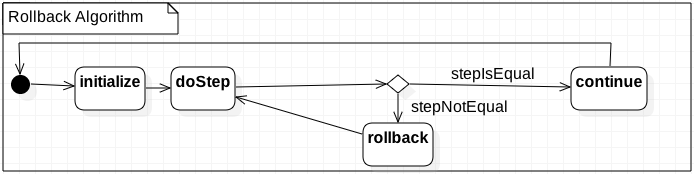
\includegraphics[width=4.5in,height=0.9in]{fig/3/MA2.png}
			\label{sd-rollback}}	
		\subfigure[可预测步长算法]{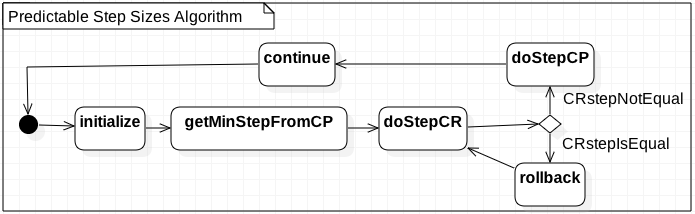
\includegraphics[width=4.5in,height=1.1in]{fig/3/MA3.png}
			\label{sd-pre}}		
	\caption{三种协同仿真主算法的活动图}
	\label{ad-fixedstep}
	}
\end{figure}
\subsubsection{固定步长算法}
对于固定步长算法,所有的FMU都有一个相同的步长。当协同仿真主算法在$t$时刻调用FMU的$doStep$函数执行步长$h$时,所有的FMU将从$t$时刻执行$h$步长并到达$t+h$时刻。在执行下一个$doStep$函数之前,要确保所有的FMU都执行完了上一个步长并且完成了数据交换。固定步长算法的活动图如图\ref{sd_fixedstep}所示,该活动图主要包含三个活动: 初始化($initialize$), 执行下一步($doStep$) 和继续执行( $continue$)。首先对所有的FMU进行初始化,之后调用$doStep$函数进行仿真,最后在$continue$活动中完成FMU之间的数据交换。 在固定步长算法中,只要保证每个FMU的仿真是可靠的,则可以保证整个仿真过程的可靠性。但是,如果在某个FMU的仿真过程中出现错误,则会导致整个协同仿真过程出错,为了解决固定步长算法的这一缺陷问题,出现了可回滚算法。
\subsubsection{可回滚算法}
FMI2.0相对于FMI1.0添加了几个重要的特性,它支持了FMU状态的保存和恢复。例如,主算法调用$FMU_{1}$和$FMU_{2}$的$doStep$函数执行$h$步长的仿真,$FMU_{1}$接受了该步长,但是$FMU_{2}$拒绝了该步长,则$FMU_{1}$和$FMU_{2}$都会先执行$h$步长的仿真然后回滚到上一个时间点。可回滚算法的活动图如图\ref{sd-rollback}所示,相比固定步长算法,可回滚算法要求所有的FMU要基于FMI2.0标准并支持$rollback$方法,且当某个FMU拒绝执行某一步长时,所有的FMU将会回滚到上一个步长执行完之后的时间点。
\subsubsection{可预测步长算法}
如果可以预测FMU下一步能执行的最大步长(FMU在不错过事件时,能执行的最长仿真时间),则可以大大提高协同仿真的效率。因此,在论文\cite{Broman2013Determinate}中,Broman David等人提出了使用$GetMaxStepSize$函数来预测FMU下一步能执行的最大步长,基于该函数的支持,他们进一步提出了可预测步长算法。图\ref{sd-pre}为可预测步长算法的活动图,首先所有的FMU进行初始化,然后支持$GetMaxStepSize$函数的FMU在$getMinStepFromCP$活动中预测他们下一步能执行的最大步长,并且在所有的最大步长中选择最小的一个$h$作为所有FMU下一步执行的步长,之后所有的FMU一起执行$h$步长,如果所有的FMU都接受了该步长,则所有的FMU都仿真该步长然后进行下一步;如果有FMU拒绝了该步长,则将所有的FMU回滚到上一个时间点,然后选择一个更小的步长进行仿真。
\subsection{协同仿真主算法的建模和可信性检测} 
\label{sec:ma}
我们用时间自动机将三种不同类型的主算法进行形式化建模,图\ref{ta-master}是三种主算法的时间自动机模型。固定步长算法的时间自动机模型包含$Init$和$doStep$两个状态,且与$FMU$的模型通过$continue$信道进行通信。 可回滚算法包括$Init$、$DoStep$和$Continue$三个状态,如果所有的FMU都接受了下一步要进行仿真的步长,则可回滚算法的时间自动机模型将发送$continue$信号,且迁移到$Continue$状态;否则,将发送$rollback$信号,且返回到上一个状态。可预测步长算法包括$Init$、 $find \_ CP \_ MIN$、$DoStep$、$writeCP$四个状态。首先他们获得支持预测步长算法的多个FMU的最大步长,并取所有最大步长的最小值$step1$ 。然后执行该步长,如果所有的FMU都接受该步长,则发送$continue$信号并迁移到下一个状态,否则发送$rollback$信号并回滚到$DoStep$状态。
\begin{figure}[htbp]
\centering{
		\subfigure[固定步长算法的时间自动机模型]{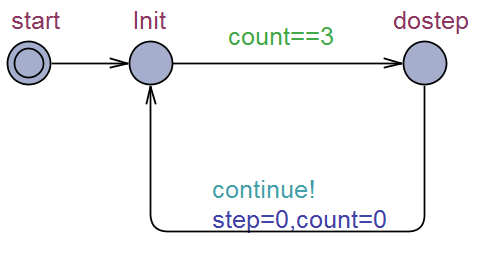
\includegraphics[width=2.0in,height=1.3in]{fig/3/fixedstep_master.png}
			\label{ta_fixedstep}}
		\hfil
		\subfigure[可回滚算法的时间自动机模型]{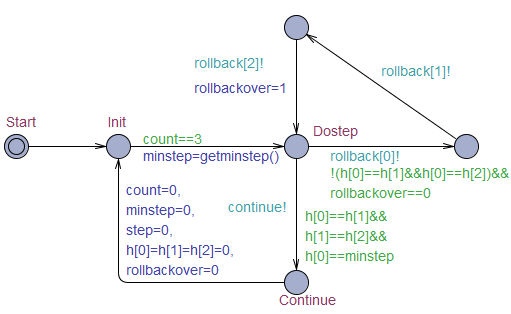
\includegraphics[width=3.0in,height=1.6in]{fig/3/rollback_master.png}
			\label{ta-rollback}}	
		\subfigure[可预测步长算法的时间自动机模型]{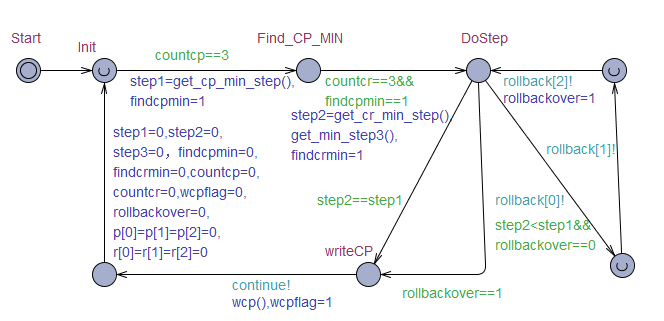
\includegraphics[width=5.0in,height=2.3in]{fig/3/pma_master.png}
			\label{ta-pre}}		
	\caption{三种不同主算法的时间自动机模型。}
	\label{ta-master}
	}
\end{figure}

UPPAAL是基于时间自动机理论对实时系统进行检测的工具,其中使用到的时间自动机模型在原始的时间自动机基础上增加了整型变量、多种数据类型及同步信号等扩展。下面我们使用UPPAAL工具对这三个主算法的可达性、活性及死锁进行检测。具体的检测属性如下所示:
\begin{itemize}
\item
$E \langle\rangle master.dostep$, $E\langle\rangle master.Continue$ and $E\langle\rangle master.writeCP$是可达性检测,用来验证这些系统状态是否可达;
\item
$master.Init -> master.dostep$, $master.Init -> master.Continue$ and $master.Init -> master.Continue$是活性检测。如果主算法可以到达前一个状态,那么它最终也会到达后一个状态。
\item
$A[] not deadlock$是死锁的检测, 用来检测主算法是否存在死锁。
\end{itemize}
实验的结果如表\ref{ta_r}所示,从表中我们可以看出模型不存在死锁,且可达性和活性都满足,说明我们的主算法是可信的。例如:属性$A[]~not~deadlock$满足,说明主算法不存在死锁; 属性$E\langle\rangle~master.doStep$ 满足,说明系统最终会到达$doStep$状态。 总结来说,我们在这一小节检测了我们所用到的协同仿真的主算法的可信性。
\begin{table}
\caption{主算法的检测结果}
\centering
\begin{tabular}{c c c}
          \hline
          主算法 & 属性 & 结果\\
       \hline
        \multirow{2}{2.0cm}{固定步长}
                & $A[]~not~deadlock$ & True\\
                & $master.Init -> master.dostep$ & True\\
                & $E\langle\rangle~master.dostep$ & True\\

        \hline
        \multirow{2}{2.0cm}{可回滚}
                & $A[]~not~deadlock$ & True\\
                & $master.Init -> master.Continue$ & True\\
                & $E\langle\rangle~master.Continue$ & True\\

        \hline
        \multirow{2}{2.0cm}{可预测}
                & $A[]~not~deadlock$ & True\\
                & $master.Init -> master.writeCP$ & True\\
                & $E\langle\rangle~master.writeCP$ & True\\
        \hline
\end{tabular}
\label{ta_r}
\end{table}

\section{系统协同仿真行为的可信性检测}
在本小节,我们使用一个水箱的案例对系统协同仿真行为的可信性检测过程进行详细的描述。由于,在检测过程中,需要用时间自动机对FMU进行形式化描述。因此,我们首先给出了从FMU到时间自动机的映射规则,然后使用SysML对整个系统进行架构设计,接下来基于FMI标准生成系统各个组件的FMU模型,并得到多个FMU之间的连接关系配置,最后我们用时间自动机建模了FMU的形式化模型,并输入到UPPAAL工具中针对多个属性进行检测分析。
\subsection{FMU到TA的映射} 
\label{sec:encode}
在本文的第二章的预备知识中,我们给出了FMU和时间自动机的语法及语义,下面我们根据第二章的语法语义给出FMU和时间自动机的映射关系。我们发现FMU和时间自动机的语义之间存在一定的关联,FMU的语义关注于FMU的执行序列,也就是状态随着时间的不断迁移,时间自动机的执行迹跟FMU的执行序列十分相似,也是状态随着时间的迁移序列。因此,我们使用时间自动机来对FMU进行形式化描述,从而来分析多个FMU之间的协同行为。
给定一个FMU$F=(S,U,Y,D,s_{0},set,get,doStep)$,我们可以根据他们执行语义之间的关联,将FMU用时间自动机$\textit{A}=(L,l_{0},E,I)$进行形式化描述:
\begin{itemize}
\item
$L$是时间自动机的有限位置集合。因此,时间自动机语义模型$L_{\textit{A}}$中的状态可以看做为FMU中的状态,即$(l,v) \Rightarrow s$。
\item
时间自动机语义模型$L_{\textit{A}}$中的初始状态可以看做为FMU中的初始状态,即$(l_{0},v_{0}) \Rightarrow s_{0}$。
\item
FMU中的输入变量$u \in U$可以看做为时间自动机的$Act_{i} \cup \{absent\}$。
\item
FMU的输出变量$y \in Y$可以看做为时间自动机的$Act_{o} \cup \{absent\}$。
\item
时间自动机的输入动作$e \in Act_{i}$可以看做FMU中的$set$函数。
\item
时间自动机的输出动作$e \in Act_{o}$可以看做为FMU中的$get$函数。  
\item
时间自动机之间依靠信道的同步可以看做为FMU之间的依赖关系。 $(u,y) \in D$表示输出变量$y$依赖于输入变量$u$,在时间自动机中输出动作同样依赖于输入动作。
\item
对于时间自动机,一个动作$e \in Act$会触发一个迁移$s \xrightarrow{e} s^{\prime}$,这个过程就相当于FMU里面的$doStep$执行,会使其到达下一个状态。 例如:时间自动机的迁移$l \xrightarrow{e} l^{\prime}$可以描述FMU的$doStep(s,h)$被调用,并且此FMU接受了步长$h$到达了下一个状态 $s^{\prime}$;然而,此FMU也可能会拒绝步长$h$,并且发生了回滚,这个过程在时间自动机里面可以用一条边$l^{\prime} \xrightarrow{e} l$进行描述,来表示回滚到了上一个状态。

\end{itemize}
\begin{figure}[htbp]
	\centering	{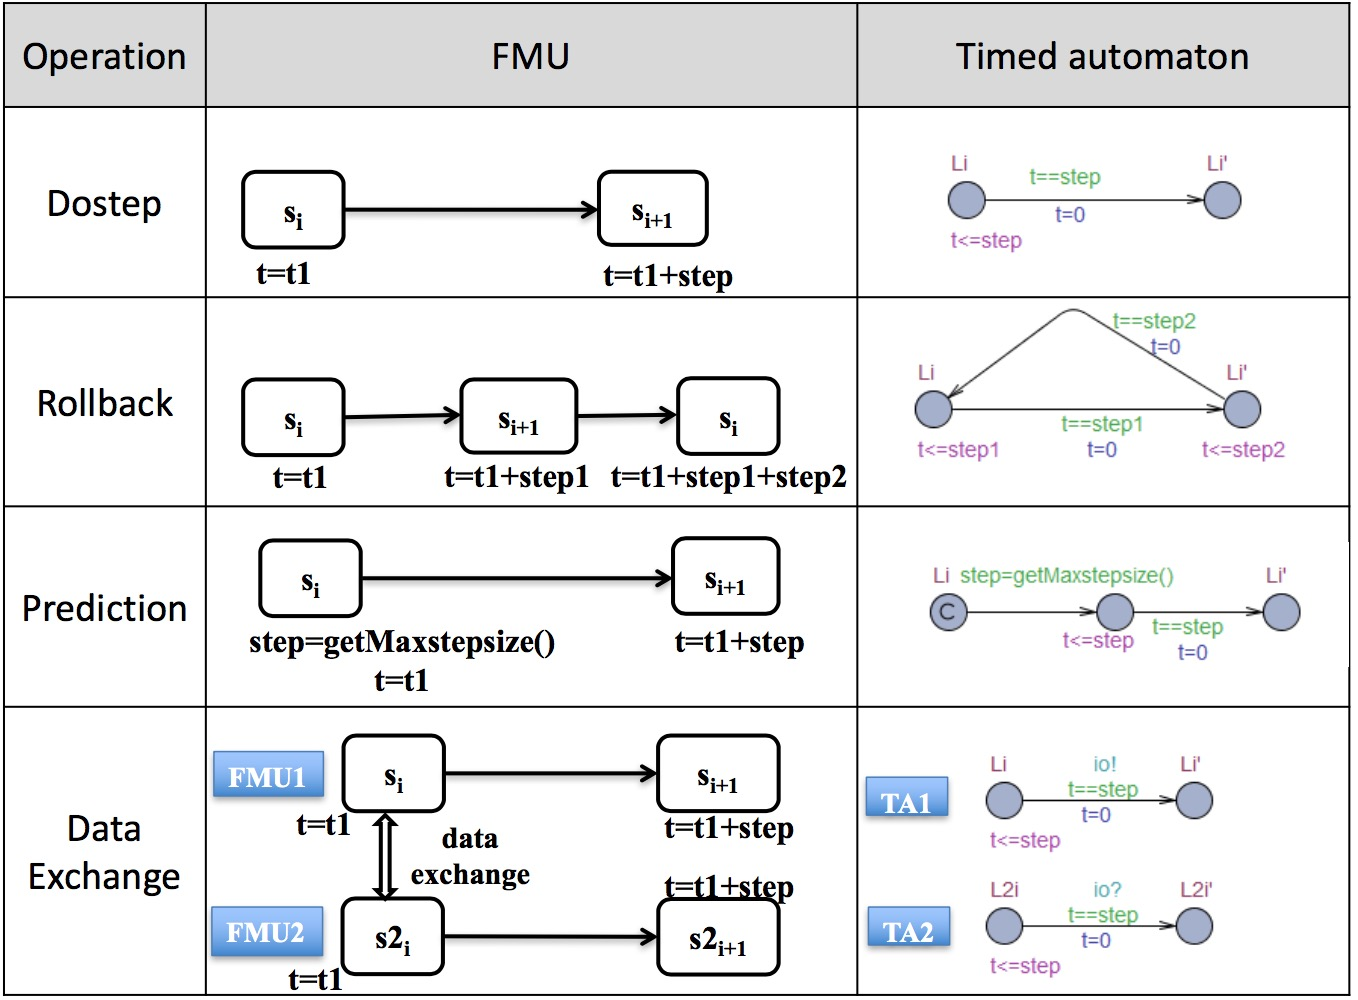
\includegraphics[width=5.0in,height=3.5in]{fig/3/abstractRole.png}}
	\caption{Encoding rules from FMU to TA.}
	\label{fmutota}
\end{figure}

将FMU直接转化为时间自动机是比较困难的,S. Tripakis曾在论文\cite{Tripakis15}中将时间自动机编码为FMU。我们受此论文的启发,根据时间自动机和FMU之间语义的关联,提出了几条在操作语义上从FMU到时间自动机的映射规则,如图\ref{fmutota}所示。
\begin{itemize}
\item
给定FMU$t_{1}$时刻的当前状态$s_{i}$,操作函数$Dostep$可以使得FMU在$t_{1}+step$时刻到达$s_{i+1}$状态。这个操作可以用时间自动机的迁移来进行表示:在位置$L_{i}$延迟$step$的时间并迁移到一个新的位置$L_{i}^{\prime}$。
\item
对于操作函数$Rollback$,给定FMU$t_{1}$时刻的当前状态$s_{i}$,FMU首先执行步长$step1$并在 $t_{1}+step1$时刻到达$s_{i+1}$状态,然后操作函数$rollback$又使得FMU回滚到上一个状态$s_{i}$。对于时间自动机来说,这个可以表示为在$L_{i}$位置延迟了$step1$时间单位并迁移到新的位置$L_{i}^{\prime}$,之后又迁移到了上一个位置$L_{i}$。 
\item
对于操作函数$Prediction$,给定一个状态$s_{i}$,FMU可以根据函数$getMaxstepsieze$得到下一步能执行的最大步长,然后执行此步长并在$t_{1}+step$时刻到达$s_{i+1}$状态。 对于时间自动机,可以表示为在$L_{i}$位置执行了一个函数并得到要延迟的时间$step$, 然后延迟该时间并迁移到一个新的位置 $L_{i}^{\prime}$ .
\item
对于操作函数$Data Exchange$,两个FMU在$t_{1}$时刻的$s_{i}$状态执行$Data Exchange$进行了数据交换,然后他们执行相同的步长并迁移到下一个位置$s_{i+1}$和$s2_{i+1}$。对于时间自动机,可以表示为两个时间自动机在$t_{1}$时刻通过信道$io$进行了同步,然后延迟了相同的时间并从$L_{i}$位置迁移到$L_{i+1}$位置。
\end{itemize}
为了将FMU用时间自动机进行形式化描述,我们提出了以上映射规则。为了证明我们以上规则的正确性,我们分析了FMU和时间自动机的执行片段如下所示:
\begin{itemize}
\item
对于操作函数$Dostep$的映射,在FMU和时间自动机中的执行片段为 ($s_{i}$, $t_{1}$),($s_{i+1}$, $t_{1}+step$)和($l_{i}$, $t$), ($l_{i}^{\prime}$, $t+step$)。这说明时间自动机和FMU都执行$step$的时间单位并到达了一个新的状态或是位置。
\item 
对于操作函数$Rollback$的映射,在FMU和时间自动机的执行片段为($s_{i}$, $t_{1}$),($s_{i+1}$, $t_{1}+step1$),($s_{i}$, $t_{1}+step1+step2$) 和 ($l_{i}$, $t$),($l_{i}^{\prime}$, $t+step1$),($l_{i}$, $t+step1+step2$)。这说明时间自动机和FMU都首先执行了$step1$时间单位,并且到达了一个新的状态或位置,然后执行了$step2$时间单位,又返回到了之前的状态或位置。
\item
对于操作函数$Prediction$的映射,FMU和时间自动机的执行片段为($s_{i}$, $t_{1}$),($s_{i+1}$, $t_{1}+step$)和($l_{i}$, $t$),($l_{i}^{\prime}$, $t+step$)。这说明时间自动机和FMU都成功预测到了步长$step$并执行了此步长。
\item
对于操作函数$Data Exchange$的映射,FMU1和时间自动机TA1的执行片段为 ($s_{i}$, $t_{1}$),($s_{i+1}$, $t_{1}+step$)和($l_{i}$, $t$),($l_{i}^{\prime}$, $t+step$)。FMU2和时间自动机TA2的执行片段为($s2_{i}$, $t_{1}$),($s2_{i+1}$, $t_{1}+step$) 和 ($l2_{i}$, $t$),($l2_{i}^{\prime}$, $t+step$)。这说明时间自动机和FMU在经过了数据交换后又执行了$step$时间单位。
\end{itemize}
为了更加准确的验证映射规则的正确性,我们分析了时间自动机和FMU的整个执行序列。我们通过分析得到FMU和时间自动机的执行序列是等价的,从而保证了映射规则的正确性。在之后几个小节的内容中,我们将此映射规则应用到了水箱的案例中,根据我们之后对案例仿真片段的分析,我们也发现该映射规则是正确的。 
\subsection{基于SysML的架构建模} 
为了更好的阐述我们的方法,我们采用了水箱的案例\cite{Am2016Checking}作为驱动以更加形象的展示我们的方法。下面我们先简单的介绍一下水箱案例,然后用SysML建模语言对整个案例的架构建模。水箱案例:有一个水源可以向水箱里面注水,且水箱里面的水通过一个管道流入到一个水池当中,这个水源的流出由一个阀门控制,而阀门的开关由一个控制器进行控制。在本小节,由于水箱、阀门、控制器连接方式的不同,我们在此描述了三种不同类型的水箱系统。

我们用SysML来建模该系统的架构,其中用SysML的BDD图来描述系统中各个组件的结构,用SysML的IBD图用来描述各个组件之间的关联关系。各个组件的接口由连接器进行关联,因此系统各个组件的依赖关系可以用各个块的接口之间的连接进行表示。

图\ref{myad}是水箱案例的SysML BDD图,其中包含三个块: $Valve$, $Tank$ 和 $Controller$。 $Valve$和$Tank$是物理组件;$Controller$是信息组件。每一个组件都有自己的输入和输出接口,例如:$Valve$的输入接口是$vin$,它用来输入阀门的开关$OpenClosed$信号。
\begin{figure}[htbp]
	\centering	{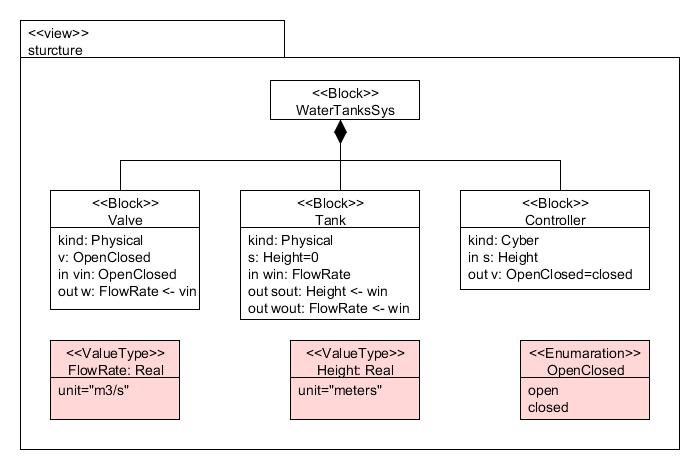
\includegraphics[width=5.0in,height=3.5in]{fig/3/AD.jpg}}
	\caption{水箱系统的SysML BDD}
	\label{myad}
\end{figure}

图\ref{cd} 是SysML的IBD图,在这里我们给出了三种连接情形。在第一种情形中,系统包含一个阀门、一个控制器和一个水箱,控制器随机的给阀门发送开关信息,导致水箱中的水位不断的变化;在第二种情形中,控制器信号的发送受到水箱水位的影响,控制器根据水箱的水位发送开关信号;在第三种情形中,我们添加了一个水箱$waterTank2$,水箱$waterTank1$中的水通过管道先流入$waterTank2$中,最后流入水池。

\begin{figure}[htbp]
\centering{
		\subfigure[情形1]{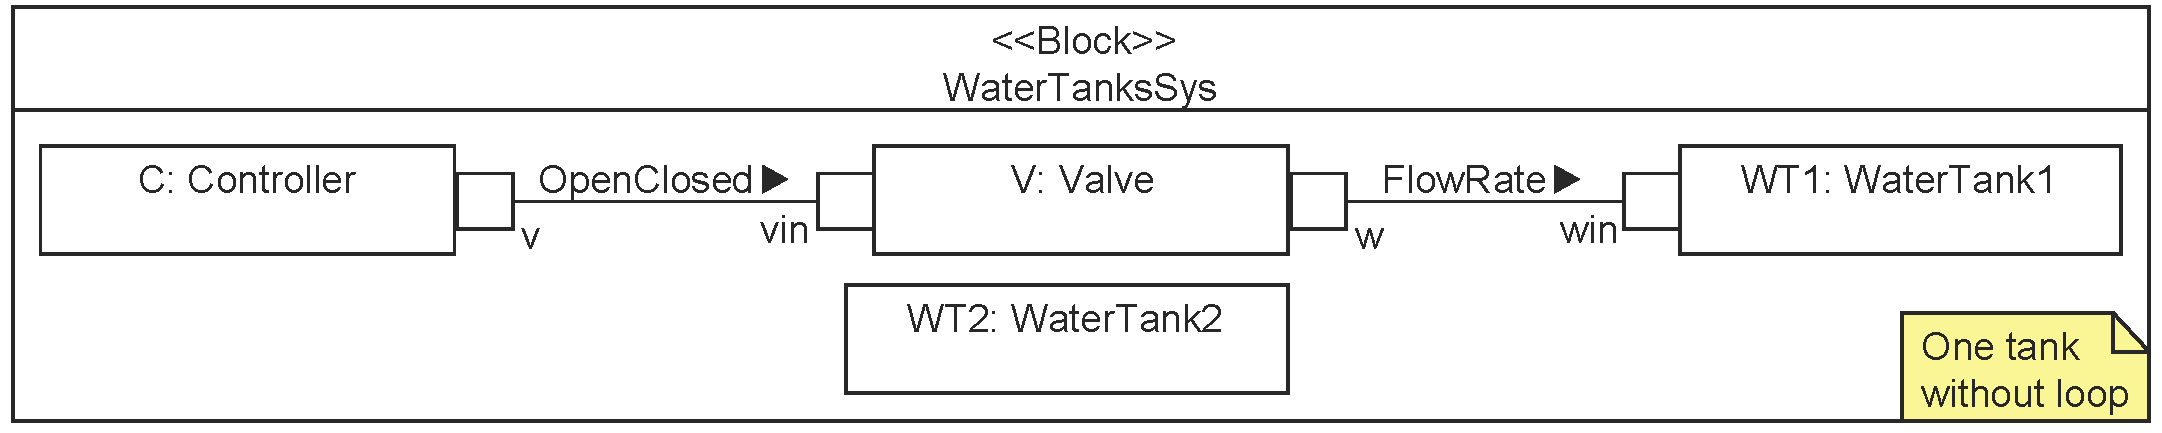
\includegraphics[width=5.0in,height=1.1in]{fig/3/CD1.png}
			\label{cd1}}
		\hfil
		\subfigure[情形2]{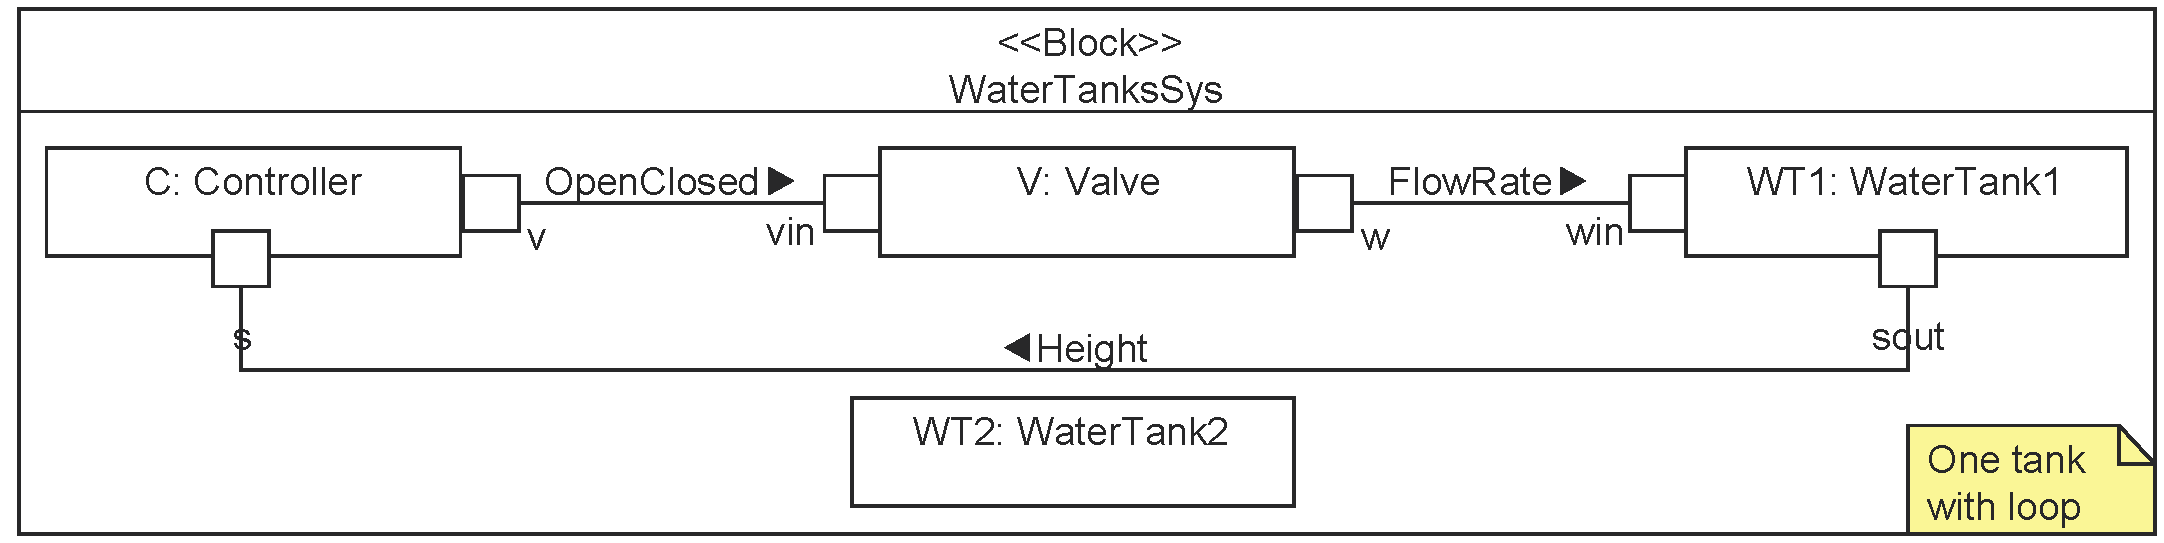
\includegraphics[width=5.0in,height=1.1in]{fig/3/CD2.png}
			\label{cd2}}
		\hfil
		\subfigure[情形3]{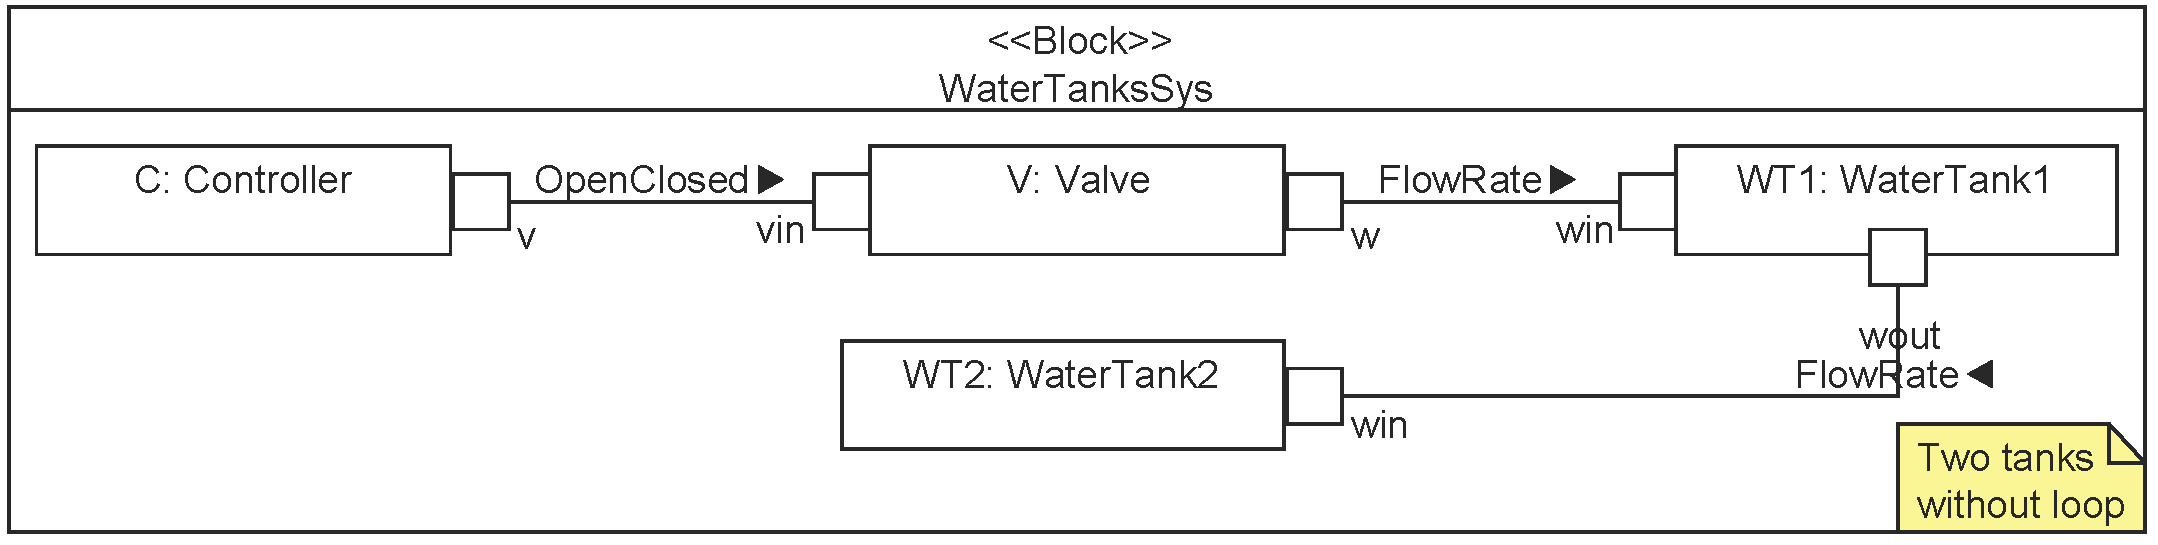
\includegraphics[width=5.0in,height=1.1in]{fig/3/CD3.png}
			\label{cd3}}
	\caption{水箱系统的SysML IBD}
	\label{cd}
	}
\end{figure}
在本小节我们用SysML BDD图描述了系统组件的结构,并用SysML的IBD图描述了各个组件之间的连接。在下一个小节,我们基于FMI标准用FMU来实现每一个系统组件,并将SysML IBD中描述的关联关系用一个FMU之间的接口配置文件进行表示。
\subsection{基于FMI的协同仿真模型设计} 
\label{sec:case}
图\ref{fmu-con}描述的是水箱系统中的FMU组件及各个FMU之间的连接。根据图\ref{cd}给定的SysML IBD,我们也得到了三种FMU的情形。第一种情形如图\ref{fmu-con1}所示,系统中有三个FMU组件:$Controller$, $Valve$ 和$WaterTank1$和两个接口$v \_ vin$及$w \_ win$。 $Controller$ 和 $Valve$由$v \_ vin$接口连接; $Valve$ 和 $WaterTank1$ 由 $w \_ win$接口连接。第二种情形如图 \ref{fmu-con2}所示,其中在第一种情形上添加了$WaterTank1$ 和$Controller$的接口$sout \_ s$,表示控制器信号的发送受到水箱$WaterTank1$的水位影响。 图\ref{fmu-con3}是第三种情形,在第一种情形上添加了另一个水箱$WaterTank2$, 水箱$WaterTank1$ 和$WaterTank2$由接口$w \_ out$连接。 
\begin{figure}[htbp]
\centering{
		\subfigure[情形1]{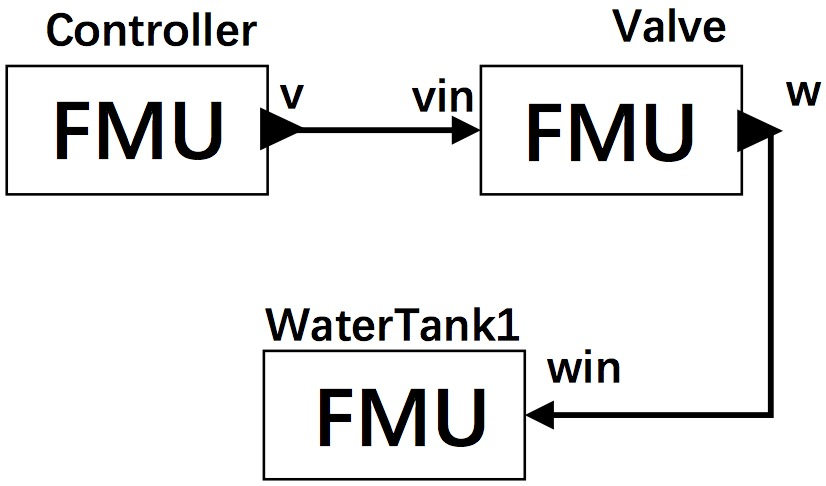
\includegraphics[width=1.5in,height=0.9in]{fig/3/fmuc1.png}
			\label{fmu-con1}}
		\hfil
		\subfigure[情形2]{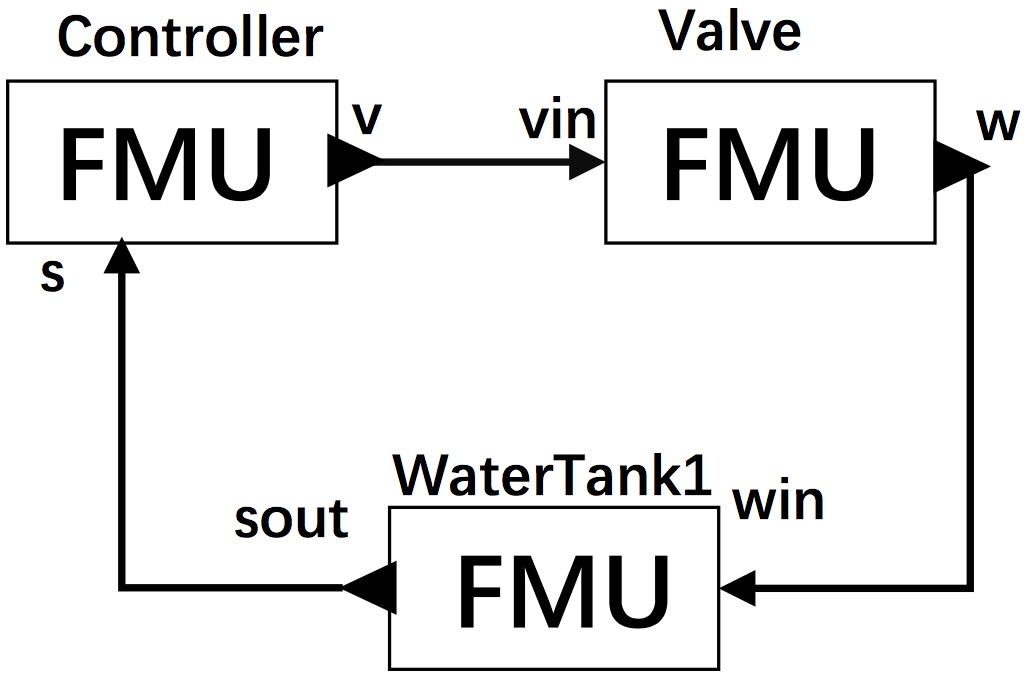
\includegraphics[width=1.5in,height=0.9in]{fig/3/fmuc2.png}
			\label{fmu-con2}}
		\hfil
		\subfigure[情形3]{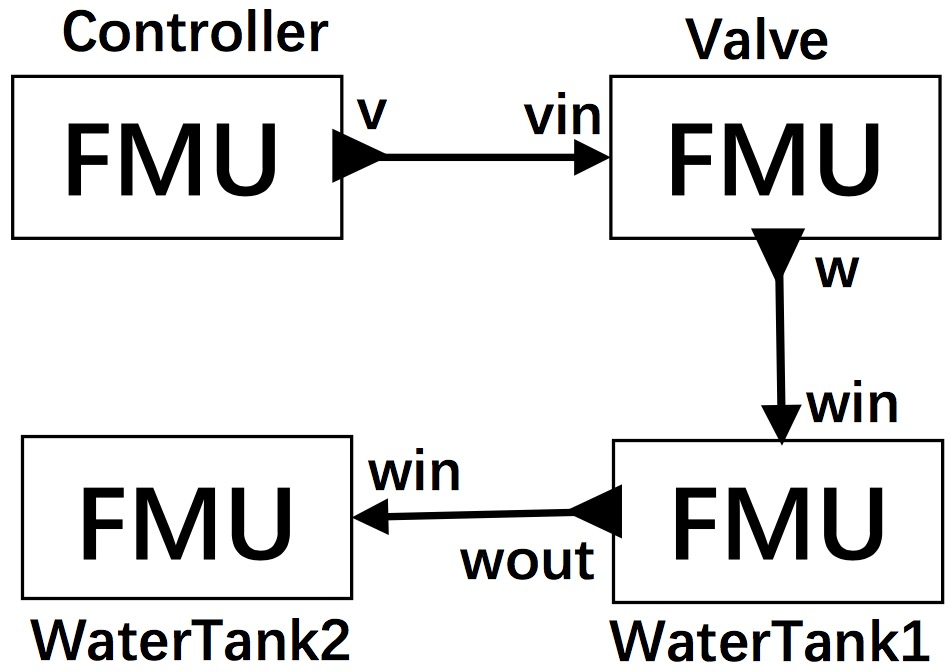
\includegraphics[width=1.5in,height=0.9in]{fig/3/fmuc3.png}
			\label{fmu-con3}}
	\caption{水箱系统中FMU的三种连接情形}
	\label{fmu-con}
	}
\end{figure}

在本小节我们设计了FMU及FMU之间的连接,我们只需要添加一个协同仿真的主算法就可以在协同仿真引擎当中对整个异构系统进行协同仿真并得到仿真迹。但是,在进行仿真之前,我们要保证各个FMU之间协同行为的正确性,因此,我们在下一个小节基于时间自动机理论对系统的协同行为进行验证,这也是我们本文的主要贡献点之一。
\subsection{协同仿真行为的可信性检测} 
\label{sec:mauppaal}
在本小节我们基于时间自动机理论对水箱系统中组件之间的协同行为的正确性进行验证。首先我们根据小节\ref{sec:encode}中提出的映射规则,将水箱系统中的FMU用时间自动机进行形式化描述,并取小节\ref{sec:ma}中建模的一个主算法(在此,采用可回滚算法作为主算法,其他算法的验证分析与该算法类似,在此不做描述),FMU之间的接口配置文件我们用时间自动机之间的信道进行描述。由此,我们得到了一个由主算法、FMU的时间自动机模型及由配置文件转化得到的信道组成的时间自动机网络。图\ref{tk-arch1}为上述小节中情形1的时间自动机网络模型。

\begin{figure}[htbp]
\centering{
		\subfigure[FMU\_controller 的时间自动机模型]{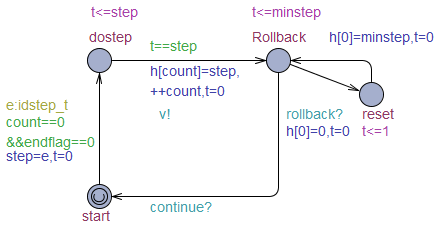
\includegraphics[width=2.5in,height=2.0in]{fig/3/2signal_controller.png}
			\label{tk_controller}}
		\hfil
		\subfigure[FMU\_valve 的时间自动机模型]{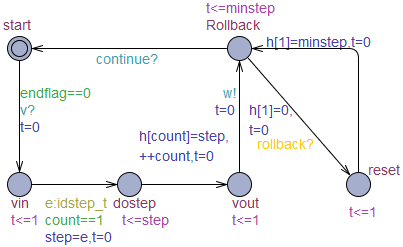
\includegraphics[width=2.5in,height=2.0in]{fig/3/2signal_v.png}
			\label{tk_v}}
			
	    \subfigure[FMU\_WaterTank1 的时间自动机模型]{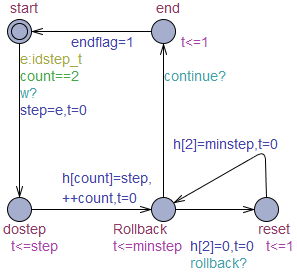
\includegraphics[width=2.2in,height=2.0in]{fig/3/2signal_wt1.png}
			\label{tk_wt1}}
		\hfil
		 \subfigure[可回滚主算法的时间自动机模型]{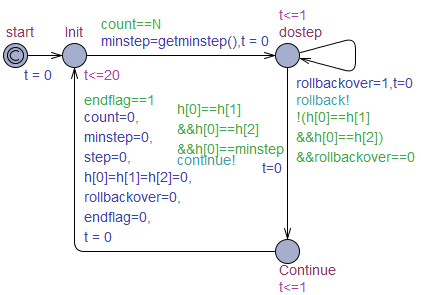
\includegraphics[width=2.8in,height=2.0in]{fig/3/2signal_master.png}
			\label{tk_ma}}		
	\caption{情形1的时间自动机网络: $controller$ $\vert\vert$ $valve$ $\vert\vert$ $WaterTank1$ $\vert\vert$ $MA$.}
	\label{tk-arch1}
	}
\end{figure}

\begin{figure}[htbp]
\centering{
		\subfigure[部分迹]{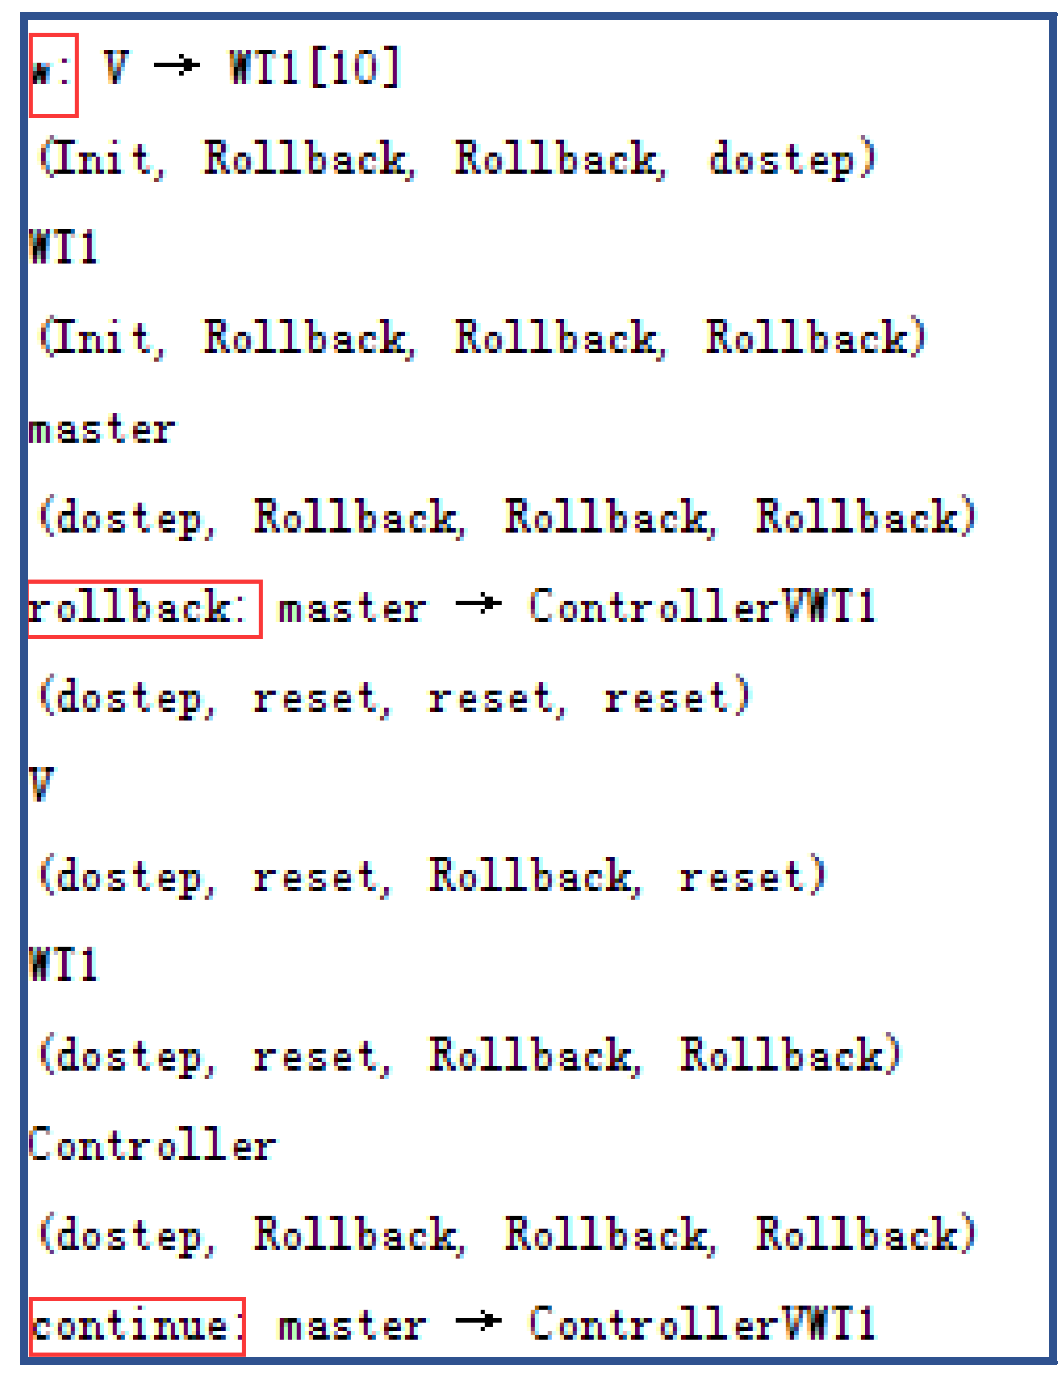
\includegraphics[width=2.5in,height=3.5in]{fig/3/trs.png}
			\label{trs}}
		\hfil
		\subfigure[执行序列图]{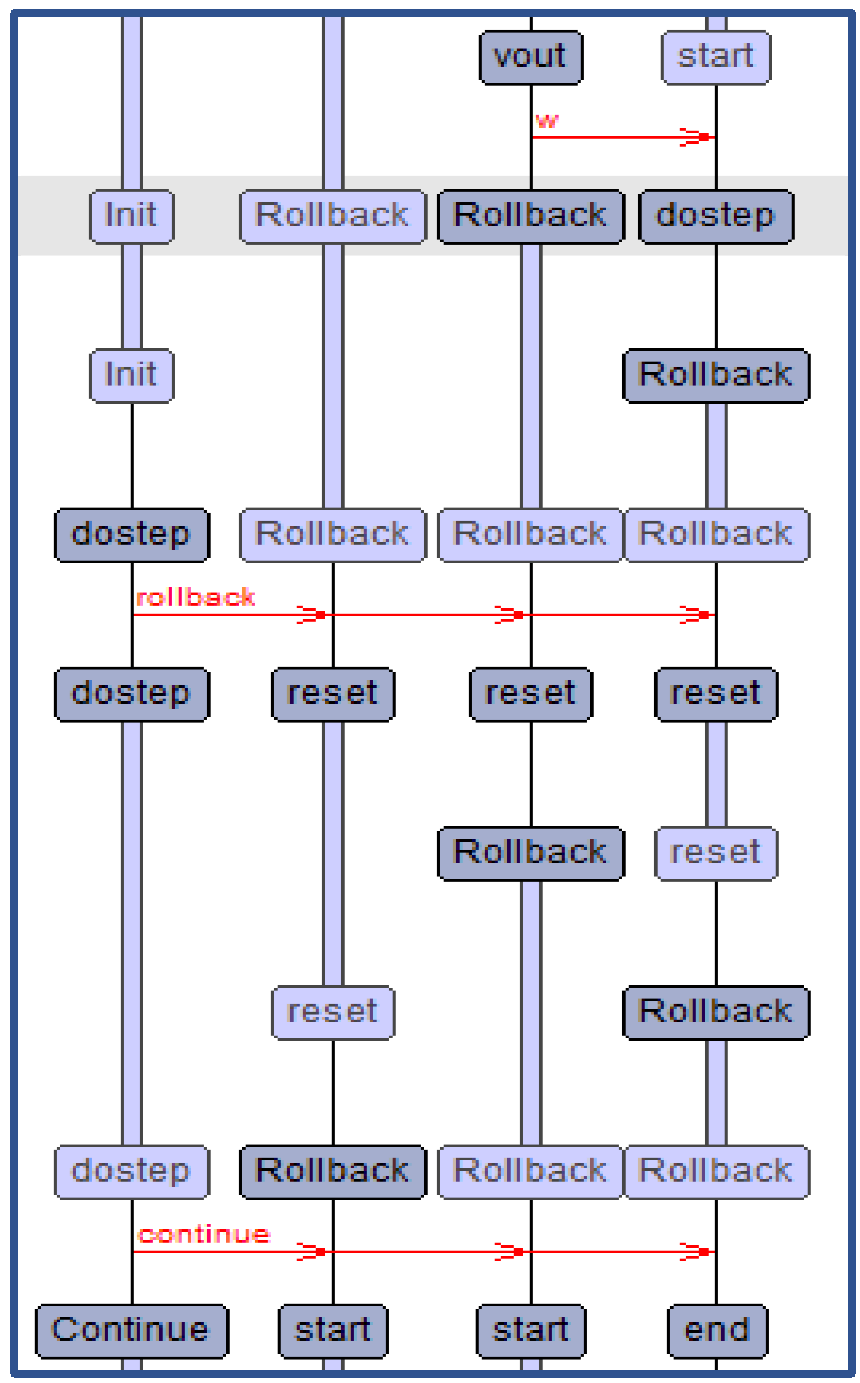
\includegraphics[width=2.5in,height=3.5in]{fig/3/seq.png}
			\label{seq}}
	\caption{协同过程在UPPAAL中的执行序列。}
	\label{trs-seq}
	}
\end{figure}

图\ref{tk_controller}, \ref{tk_v}, \ref{tk_wt1}分别是$controller$, $valve$ 和 $WaterTank1$的时间自动机模型。这些自动机都有四个主要的位置:$start$, $dostep$, $Rollback$和$reset$。图\ref{tk_controller}是 $controller$的时间自动机模型,它首先通过信道 $v$与$valve$的时间自动机模型进行交互并到达$Rollback$状态,然后等待主算法的信号,直到它收到了来自主算法的$continue$信号再与其他的FMU进行数据交互并到达$start$状态;否则,它收到$rollback$信号,并回到$Rollback$状态。$valve$和$WaterTank1$的时间自动机中位置和迁移与 $controller$类似。图\ref{tk_ma} 是主算法的时间自动机模型,首先主算法先进性参数初始化,然后根据条件来判断发出  $continue$信号或是$rollback$信号。

图\ref{trs-seq}是协同过程在UPPAAL中的执行片段,我们可以看到 $valve$ 首先发送了信号$w$ 来与 $WaterTank1$进行数据交换,然后,$WaterTank1$ 到达了 $dostep$ 状态,之后主算法广播  $rollback$信号导致FMU到达$reset$状态,最后主算法发送$continue$ 信号使得所有的FMU到达 $start$状态并开始下一步仿真。通过对执行序列的分析,我们发现模型可以正确仿真。

为了比较小节\ref{sec:case}中描述的三种情形的协同行为,我们同时用时间自动机形式化描述了其他两种情形。对于第二种情形,我们在第一种情形基础上添加了$controller$ 和 $WaterTank1$之间的信道$s$如图\ref{tk-arch2}所示;对于第三种情形我们建模了$WaterTank2$的模型并添加了信道$w2$ 如图Fig.\ref{arc3}所示。其他的模型与第一种情形中的模型类似,我们在此只给出了新增加的或有改动的模型。接下来我们将对这三种情形进行验证。
\begin{figure}[htbp]
\centering{
		\subfigure[TA for FMU\_controller]{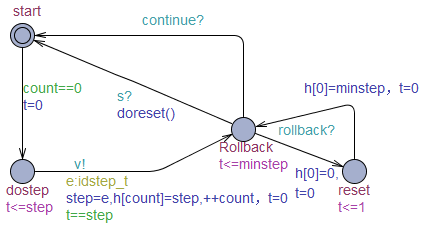
\includegraphics[width=2.7in,height=2.0in]{fig/3/2signal_cycle_controller.png}
			\label{tk2_controller}}
		\hfil
		\subfigure[TA for FMU\_WaterTank1]{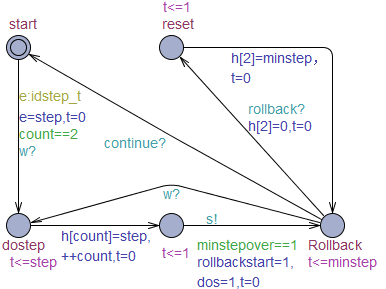
\includegraphics[width=2.3in,height=2.0in]{fig/3/2signal_cycle_wt1.png}
			\label{tk2_v}}		
	\caption{TA for connection case 2.}
	\label{tk-arch2}
	}
\end{figure}
\begin{figure}[htbp]
	\centering	{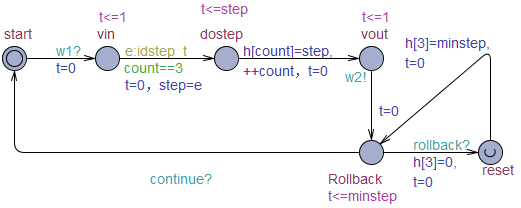
\includegraphics[width=5.0in,height=2.0in]{fig/3/4signal_wt2.png}}
	\caption{TA for FMU\_WaterTank2 of connection case 3.}\label{arc3}
\end{figure}

\begin{table}
\caption{三种情形的验证结果}
\centering
\begin{tabular}{c c c} 
        \hline  
        情形 & 验证属性 & 结果\\
        \hline
        \multirow{2}{2.0cm}{情形1}  
                & $E\langle\rangle~WT1.Rollback$ & True\\ 
                & $E\langle\rangle~master.Continue$ & True\\ 
                & $master.start -> master.Continue$ & True\\ 
                & $A[]~not~deadlock$ & True\\   
        \hline 
        \multirow{2}{2.0cm}{情形2}  
                & $E\langle\rangle~WT1.Rollback$ & True\\ 
                & $E\langle\rangle~master.Continue$ & False\\ 
                & $master.start -> master.Continue$ & False\\ 
                & $A[]~not~deadlock$ & True\\   
        \hline 
        \multirow{2}{2.0cm}{情形3}  
                & $E\langle\rangle~WT1.Rollback$ & True\\ 
                & $E\langle\rangle~master.Continue$ & True\\ 
                & $master.start -> master.Continue$ & True\\ 
                & $A[]~not~deadlock$ & True\\   
        \hline 
\end{tabular} 
\label{rs}
\end{table}

我们对每一种情形都验证了以下属性:
\begin{itemize}
\item
$E\langle\rangle~WT1.Rollback$和 $E\langle\rangle~master.Continue$ 为可达性验证,它表示$WaterTank1$将到达$Rollback$状态 且主算法会到达 $Continue$状态。
\item
$master.start -> master.Continue$为活性验证,它表示一旦主算法开始,它最早会到达 $Continue$状态.
\item 
$A[]~not~deadlock$为死锁的验证,它用来验证系统有无死锁。
\end{itemize}

验证结果如表\ref{rs}所示,我们发现情形1和情形3的验证属性都满足,它表示该情形的协同是正确的。然而情形2的可达性和活性不满足,是由于在该模型中出现了环路依赖,我们需要消除该环路依赖再进行下一步的仿真,在本文中我们只关注协同行为的验证,对于如何消除环路依赖在接下来的工作中我们会做进一步研究。 


\section{本章小结}
在本小节我们提出了一种新的方法来验证异构系统协同行为的正确性,我们首先用SysML建模语言建模了整个系统的架构,然后基于FMI标准对整个架构进行实现。之后提出了一种映射规则将FMU用时间自动机进行了形式化描述,最后基于时间自动机理论对整个系统的协同行为的正确性进行了验证。经过本小节的验证,我们可以得到通过验证的基于FMI标准的模型,该模型可以在协同仿真引擎中直接仿真并得到仿真迹,在下一个小节,我们将提出一种高效的统计模型检测方法,针对某些验证属性对协同仿真的迹进行定量的评估。